\documentclass[twoside]{book}

% Packages required by doxygen
\usepackage{fixltx2e}
\usepackage{calc}
\usepackage{doxygen}
\usepackage[export]{adjustbox} % also loads graphicx
\usepackage{graphicx}
\usepackage[utf8]{inputenc}
\usepackage{makeidx}
\usepackage{multicol}
\usepackage{multirow}
\PassOptionsToPackage{warn}{textcomp}
\usepackage{textcomp}
\usepackage[nointegrals]{wasysym}
\usepackage[table]{xcolor}

% Font selection
\usepackage[T1]{fontenc}
\usepackage[scaled=.90]{helvet}
\usepackage{courier}
\usepackage{amssymb}
\usepackage{sectsty}
\renewcommand{\familydefault}{\sfdefault}
\allsectionsfont{%
  \fontseries{bc}\selectfont%
  \color{darkgray}%
}
\renewcommand{\DoxyLabelFont}{%
  \fontseries{bc}\selectfont%
  \color{darkgray}%
}
\newcommand{\+}{\discretionary{\mbox{\scriptsize$\hookleftarrow$}}{}{}}

% Page & text layout
\usepackage{geometry}
\geometry{%
  a4paper,%
  top=2.5cm,%
  bottom=2.5cm,%
  left=2.5cm,%
  right=2.5cm%
}
\tolerance=750
\hfuzz=15pt
\hbadness=750
\setlength{\emergencystretch}{15pt}
\setlength{\parindent}{0cm}
\setlength{\parskip}{3ex plus 2ex minus 2ex}
\makeatletter
\renewcommand{\paragraph}{%
  \@startsection{paragraph}{4}{0ex}{-1.0ex}{1.0ex}{%
    \normalfont\normalsize\bfseries\SS@parafont%
  }%
}
\renewcommand{\subparagraph}{%
  \@startsection{subparagraph}{5}{0ex}{-1.0ex}{1.0ex}{%
    \normalfont\normalsize\bfseries\SS@subparafont%
  }%
}
\makeatother

% Headers & footers
\usepackage{fancyhdr}
\pagestyle{fancyplain}
\fancyhead[LE]{\fancyplain{}{\bfseries\thepage}}
\fancyhead[CE]{\fancyplain{}{}}
\fancyhead[RE]{\fancyplain{}{\bfseries\leftmark}}
\fancyhead[LO]{\fancyplain{}{\bfseries\rightmark}}
\fancyhead[CO]{\fancyplain{}{}}
\fancyhead[RO]{\fancyplain{}{\bfseries\thepage}}
\fancyfoot[LE]{\fancyplain{}{}}
\fancyfoot[CE]{\fancyplain{}{}}
\fancyfoot[RE]{\fancyplain{}{\bfseries\scriptsize Generated by Doxygen }}
\fancyfoot[LO]{\fancyplain{}{\bfseries\scriptsize Generated by Doxygen }}
\fancyfoot[CO]{\fancyplain{}{}}
\fancyfoot[RO]{\fancyplain{}{}}
\renewcommand{\footrulewidth}{0.4pt}
\renewcommand{\chaptermark}[1]{%
  \markboth{#1}{}%
}
\renewcommand{\sectionmark}[1]{%
  \markright{\thesection\ #1}%
}

% Indices & bibliography
\usepackage{natbib}
\usepackage[titles]{tocloft}
\setcounter{tocdepth}{3}
\setcounter{secnumdepth}{5}
\makeindex

% Hyperlinks (required, but should be loaded last)
\usepackage{ifpdf}
\ifpdf
  \usepackage[pdftex,pagebackref=true]{hyperref}
\else
  \usepackage[ps2pdf,pagebackref=true]{hyperref}
\fi
\hypersetup{%
  colorlinks=true,%
  linkcolor=blue,%
  citecolor=blue,%
  unicode%
}

% Custom commands
\newcommand{\clearemptydoublepage}{%
  \newpage{\pagestyle{empty}\cleardoublepage}%
}

\usepackage{caption}
\captionsetup{labelsep=space,justification=centering,font={bf},singlelinecheck=off,skip=4pt,position=top}

%===== C O N T E N T S =====

\begin{document}

% Titlepage & ToC
\hypersetup{pageanchor=false,
             bookmarksnumbered=true,
             pdfencoding=unicode
            }
\pagenumbering{alph}
\begin{titlepage}
\vspace*{7cm}
\begin{center}%
{\Large My Project }\\
\vspace*{1cm}
{\large Generated by Doxygen 1.8.13}\\
\end{center}
\end{titlepage}
\clearemptydoublepage
\pagenumbering{roman}
\tableofcontents
\clearemptydoublepage
\pagenumbering{arabic}
\hypersetup{pageanchor=true}

%--- Begin generated contents ---
\chapter{R\+E\+A\+D\+ME}
\label{md_README}
\Hypertarget{md_README}
Use the Makefile then enter ./exec to execute the program. When the graphical interfasse is open, press any key to start the sort and wait until the end of the animation. When the sort finishes press any key to close the application. 
\chapter{Class Index}
\section{Class List}
Here are the classes, structs, unions and interfaces with brief descriptions\+:\begin{DoxyCompactList}
\item\contentsline{section}{\hyperlink{classnoeud}{noeud} }{\pageref{classnoeud}}{}
\end{DoxyCompactList}

\chapter{File Index}
\section{File List}
Here is a list of all documented files with brief descriptions\+:\begin{DoxyCompactList}
\item\contentsline{section}{\hyperlink{affichage_8cpp}{affichage.\+cpp} \\*Fichier d\textquotesingle{}affichage }{\pageref{affichage_8cpp}}{}
\item\contentsline{section}{{\bfseries affichage.\+h} }{\pageref{affichage_8h}}{}
\item\contentsline{section}{\hyperlink{visu_8cpp}{visu.\+cpp} \\*Traitement du graphe }{\pageref{visu_8cpp}}{}
\item\contentsline{section}{{\bfseries visu.\+h} }{\pageref{visu_8h}}{}
\end{DoxyCompactList}

\chapter{Class Documentation}
\hypertarget{classnoeud}{}\section{noeud Class Reference}
\label{classnoeud}\index{noeud@{noeud}}


Collaboration diagram for noeud\+:
\nopagebreak
\begin{figure}[H]
\begin{center}
\leavevmode
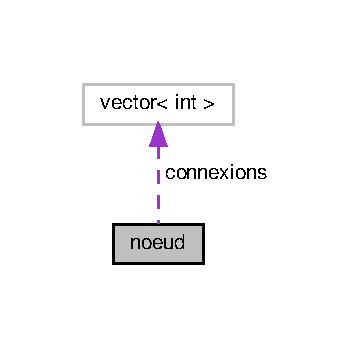
\includegraphics[width=169pt]{classnoeud__coll__graph}
\end{center}
\end{figure}
\subsection*{Public Member Functions}
\begin{DoxyCompactItemize}
\item 
\mbox{\Hypertarget{classnoeud_a1fceeeadf0a50a0e939547f4cd9bd204}\label{classnoeud_a1fceeeadf0a50a0e939547f4cd9bd204}} 
{\bfseries noeud} (int id, int x, int y, vector$<$ int $>$ connexions)
\end{DoxyCompactItemize}
\subsection*{Public Attributes}
\begin{DoxyCompactItemize}
\item 
\mbox{\Hypertarget{classnoeud_afe9e88272d7aba8cf7462046a97be26a}\label{classnoeud_afe9e88272d7aba8cf7462046a97be26a}} 
int {\bfseries id}
\item 
\mbox{\Hypertarget{classnoeud_a08c566e34f51ca6d6e3c8f20f6318a8e}\label{classnoeud_a08c566e34f51ca6d6e3c8f20f6318a8e}} 
int {\bfseries x}
\item 
\mbox{\Hypertarget{classnoeud_a85bdb2c0ee612f23d28e5e5c2c62cb67}\label{classnoeud_a85bdb2c0ee612f23d28e5e5c2c62cb67}} 
int {\bfseries y}
\item 
\mbox{\Hypertarget{classnoeud_a424c782cc730a5200c2783e64a7aa6e1}\label{classnoeud_a424c782cc730a5200c2783e64a7aa6e1}} 
vector$<$ int $>$ {\bfseries connexions}
\end{DoxyCompactItemize}


The documentation for this class was generated from the following file\+:\begin{DoxyCompactItemize}
\item 
visu.\+h\end{DoxyCompactItemize}

\chapter{File Documentation}
\hypertarget{affichage_8cpp}{}\section{affichage.\+cpp File Reference}
\label{affichage_8cpp}\index{affichage.\+cpp@{affichage.\+cpp}}


fichier d\textquotesingle{}affichage  


{\ttfamily \#include $<$iostream$>$}\newline
{\ttfamily \#include $<$vector$>$}\newline
{\ttfamily \#include $<$string$>$}\newline
{\ttfamily \#include $<$math.\+h$>$}\newline
{\ttfamily \#include $<$time.\+h$>$}\newline
{\ttfamily \#include $<$unistd.\+h$>$}\newline
{\ttfamily \#include $<$random$>$}\newline
{\ttfamily \#include $<$chrono$>$}\newline
{\ttfamily \#include $<$S\+D\+L/\+S\+D\+L.\+h$>$}\newline
{\ttfamily \#include \char`\"{}affichage.\+h\char`\"{}}\newline
{\ttfamily \#include \char`\"{}visu.\+h\char`\"{}}\newline
Include dependency graph for affichage.\+cpp\+:
\nopagebreak
\begin{figure}[H]
\begin{center}
\leavevmode
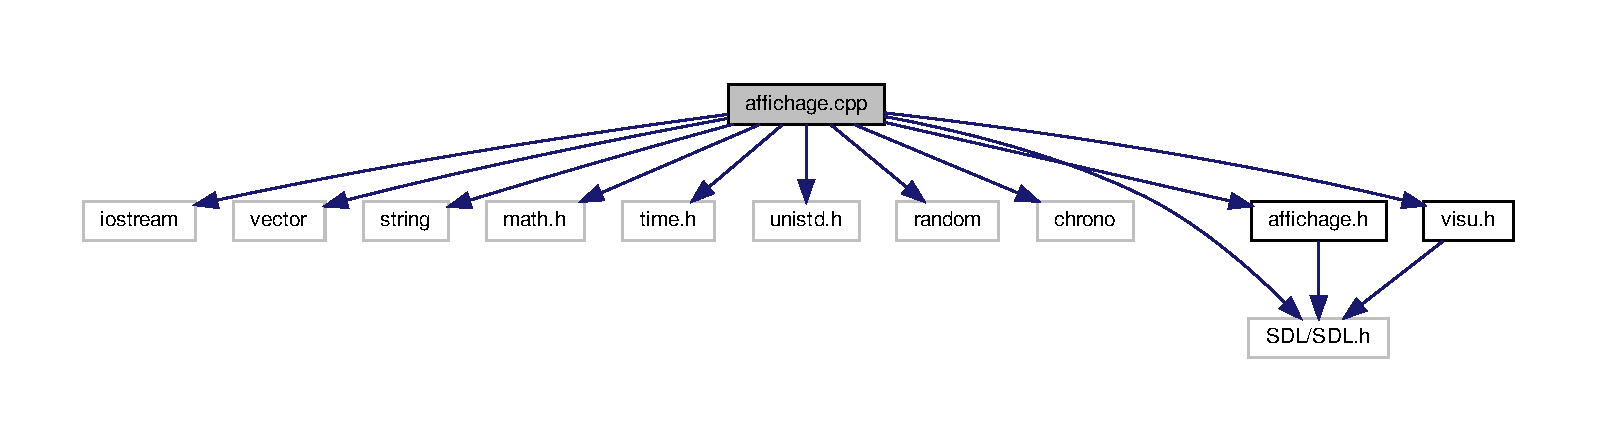
\includegraphics[width=350pt]{affichage_8cpp__incl}
\end{center}
\end{figure}
\subsection*{Functions}
\begin{DoxyCompactItemize}
\item 
\mbox{\Hypertarget{affichage_8cpp_ae2c8ce5c0d49c2a2bdb2c6eaa012d004}\label{affichage_8cpp_ae2c8ce5c0d49c2a2bdb2c6eaa012d004}} 
void {\bfseries init\+S\+DL} (S\+D\+L\+\_\+\+Surface $\ast$$\ast$screen)
\item 
\mbox{\Hypertarget{affichage_8cpp_afaa1926a40fb24056ffe955ef3d5c8d4}\label{affichage_8cpp_afaa1926a40fb24056ffe955ef3d5c8d4}} 
void {\bfseries attendre\+Touche} (void)
\item 
\mbox{\Hypertarget{affichage_8cpp_afa26708d2c8eb3e7a5e6f904a6855e7f}\label{affichage_8cpp_afa26708d2c8eb3e7a5e6f904a6855e7f}} 
void {\bfseries echanger\+Entiers} (int $\ast$x, int $\ast$y)
\item 
\mbox{\Hypertarget{affichage_8cpp_a2d806f06166e3c8426df3b8d6c65ff88}\label{affichage_8cpp_a2d806f06166e3c8426df3b8d6c65ff88}} 
void {\bfseries set\+Pixel} (int x, int y, Uint32 coul, S\+D\+L\+\_\+\+Surface $\ast$screen)
\item 
\mbox{\Hypertarget{affichage_8cpp_a3d0747c7899f5ee416d4b06727985ebb}\label{affichage_8cpp_a3d0747c7899f5ee416d4b06727985ebb}} 
void {\bfseries set\+Pixel\+Verif} (int x, int y, Uint32 coul, S\+D\+L\+\_\+\+Surface $\ast$screen)
\item 
\mbox{\Hypertarget{affichage_8cpp_a4c2ffc4b8fcf64d9ea23a06852d49cd4}\label{affichage_8cpp_a4c2ffc4b8fcf64d9ea23a06852d49cd4}} 
void {\bfseries ligne} (int x1, int y1, int x2, int y2, S\+D\+L\+\_\+\+Surface $\ast$screen)
\item 
\mbox{\Hypertarget{affichage_8cpp_a5081c1e3fc245c8f452761b23fa25407}\label{affichage_8cpp_a5081c1e3fc245c8f452761b23fa25407}} 
void {\bfseries ligne\+Horizontale} (int x, int y, int w, Uint32 coul, S\+D\+L\+\_\+\+Surface $\ast$screen)
\item 
\mbox{\Hypertarget{affichage_8cpp_aa2940066793788c9d9f5acaec416af35}\label{affichage_8cpp_aa2940066793788c9d9f5acaec416af35}} 
void {\bfseries cercle} (int cx, int cy, int rayon, S\+D\+L\+\_\+\+Surface $\ast$screen)
\end{DoxyCompactItemize}


\subsection{Detailed Description}
fichier d\textquotesingle{}affichage 

\begin{DoxyAuthor}{Author}
Aness M\+E\+N\+AA 
\end{DoxyAuthor}

\hypertarget{visu_8cpp}{}\section{visu.\+cpp File Reference}
\label{visu_8cpp}\index{visu.\+cpp@{visu.\+cpp}}


Traitement du graphe.  


{\ttfamily \#include $<$iostream$>$}\newline
{\ttfamily \#include $<$vector$>$}\newline
{\ttfamily \#include $<$string$>$}\newline
{\ttfamily \#include $<$math.\+h$>$}\newline
{\ttfamily \#include $<$time.\+h$>$}\newline
{\ttfamily \#include $<$unistd.\+h$>$}\newline
{\ttfamily \#include $<$random$>$}\newline
{\ttfamily \#include $<$chrono$>$}\newline
{\ttfamily \#include $<$S\+D\+L/\+S\+D\+L.\+h$>$}\newline
{\ttfamily \#include \char`\"{}affichage.\+h\char`\"{}}\newline
{\ttfamily \#include \char`\"{}visu.\+h\char`\"{}}\newline
Include dependency graph for visu.\+cpp\+:
\nopagebreak
\begin{figure}[H]
\begin{center}
\leavevmode
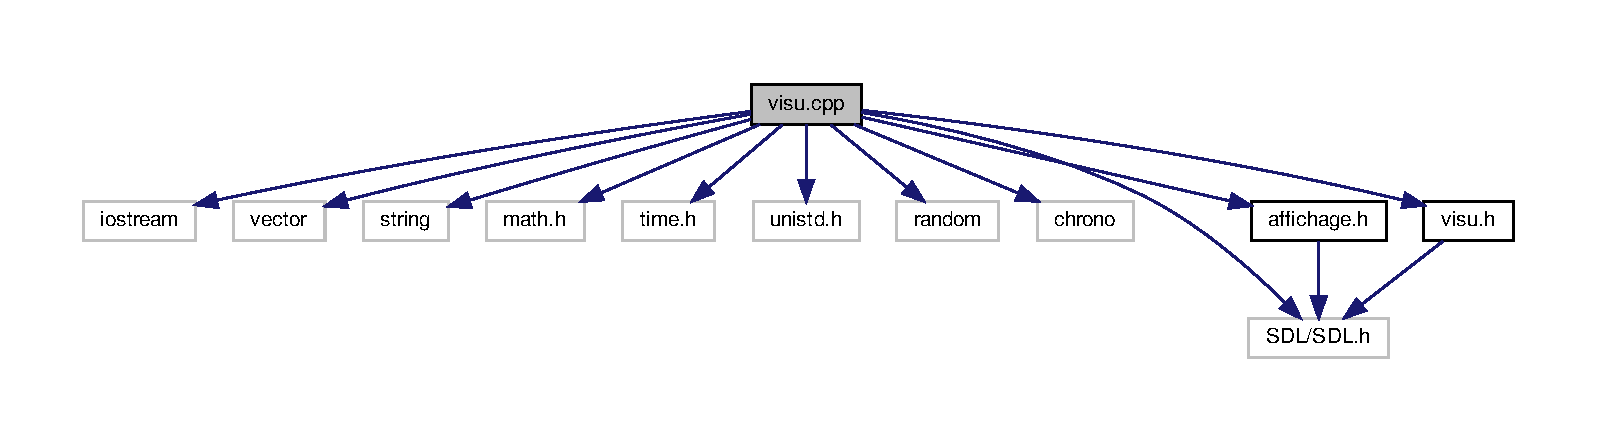
\includegraphics[width=350pt]{visu_8cpp__incl}
\end{center}
\end{figure}
\subsection*{Functions}
\begin{DoxyCompactItemize}
\item 
vector$<$ int $>$ \hyperlink{visu_8cpp_abd0c5a20ad8a89156c20efda37a90f94}{vector\+Connexions} (int nalea)
\begin{DoxyCompactList}\small\item\em Génère la position aléatoirement des noeuds. \end{DoxyCompactList}\item 
void \hyperlink{visu_8cpp_a4b02b45a77911230876c885a967d3d59}{my\+\_\+delay} (int i)
\begin{DoxyCompactList}\small\item\em Temporisation de l\textquotesingle{}animation. \end{DoxyCompactList}\item 
int \hyperlink{visu_8cpp_a165d3a2b6f41d7f3d9b4e56e83c38caa}{test\+Inside} (int x, int y, S\+D\+L\+\_\+\+Surface $\ast$screen)
\begin{DoxyCompactList}\small\item\em Teste si le noeud est dans l\textquotesingle{}écran. \end{DoxyCompactList}\item 
int \hyperlink{visu_8cpp_aaa9a2282aca02d1d0240136996bbd589}{proche} (\hyperlink{classnoeud}{noeud} $\ast$n1, \hyperlink{classnoeud}{noeud} $\ast$n2)
\begin{DoxyCompactList}\small\item\em Teste si deux noeud sont proche l\textquotesingle{}un de l\textquotesingle{}autre. \end{DoxyCompactList}\item 
void \hyperlink{visu_8cpp_aac465951eaf052e3fff82605ec4292b0}{alg\+Rapprochement} (\hyperlink{classnoeud}{noeud} $\ast$n1, \hyperlink{classnoeud}{noeud} $\ast$n2, S\+D\+L\+\_\+\+Surface $\ast$screen)
\begin{DoxyCompactList}\small\item\em Fonction se chargent de rapprocher les deux noeuds mis en argument. \end{DoxyCompactList}\item 
void \hyperlink{visu_8cpp_ad11ef364e45e6bec18158c71e5fa90aa}{alg\+Eloignement\+Proche} (\hyperlink{classnoeud}{noeud} $\ast$n1, \hyperlink{classnoeud}{noeud} $\ast$n2, S\+D\+L\+\_\+\+Surface $\ast$screen)
\begin{DoxyCompactList}\small\item\em Fonction se chargent d\textquotesingle{}éloigner les deux noeuds mis en argument. \end{DoxyCompactList}\item 
int \hyperlink{visu_8cpp_a9345b36f8d396752014bbfbad9a5f1de}{attraction} (\hyperlink{classnoeud}{noeud} $\ast$n1, \hyperlink{classnoeud}{noeud} $\ast$n2, S\+D\+L\+\_\+\+Surface $\ast$screen)
\begin{DoxyCompactList}\small\item\em Calcule l\textquotesingle{}attaction entre deux noeuds. \end{DoxyCompactList}\item 
int \hyperlink{visu_8cpp_a3e8102cdd5e1c16e0d42dd4d8c5c5beb}{repultion\+Proche} (\hyperlink{classnoeud}{noeud} $\ast$n1, \hyperlink{classnoeud}{noeud} $\ast$n2, S\+D\+L\+\_\+\+Surface $\ast$screen)
\begin{DoxyCompactList}\small\item\em Calcule la répultion entre deux noeuds. \end{DoxyCompactList}\item 
vector$<$ \hyperlink{classnoeud}{noeud} $>$ \hyperlink{visu_8cpp_a5ca74eaf1ae9b5ac15cf093a4622e207}{creat\+Graph\+Alea} ()
\begin{DoxyCompactList}\small\item\em Génère un graphe aléatoire. \end{DoxyCompactList}\item 
\mbox{\Hypertarget{visu_8cpp_aa25372c78da37b42b6be75bd30c265be}\label{visu_8cpp_aa25372c78da37b42b6be75bd30c265be}} 
vector$<$ \hyperlink{classnoeud}{noeud} $>$ \hyperlink{visu_8cpp_aa25372c78da37b42b6be75bd30c265be}{creat\+Graph} ()
\begin{DoxyCompactList}\small\item\em Création d\textquotesingle{}un Graphe de teste. \end{DoxyCompactList}\item 
void \hyperlink{visu_8cpp_a0c98fe54caf74d4a00866bc835d53519}{affiche\+Graph} (vector$<$ \hyperlink{classnoeud}{noeud} $>$ graph, S\+D\+L\+\_\+\+Surface $\ast$screen)
\begin{DoxyCompactList}\small\item\em Affichage de l\textquotesingle{}interface graphique. \end{DoxyCompactList}\item 
void \hyperlink{visu_8cpp_a338fd44c440fbc64d7f372b5595be090}{visualisation} (S\+D\+L\+\_\+\+Surface $\ast$$\ast$screen, vector$<$ \hyperlink{classnoeud}{noeud} $>$ $\ast$g)
\begin{DoxyCompactList}\small\item\em Calcule et mise à jour de l\textquotesingle{}interface graphique. \end{DoxyCompactList}\end{DoxyCompactItemize}


\subsection{Detailed Description}
Traitement du graphe. 

\begin{DoxyAuthor}{Author}
Aness M\+E\+N\+AA 
\end{DoxyAuthor}


\subsection{Function Documentation}
\mbox{\Hypertarget{visu_8cpp_a0c98fe54caf74d4a00866bc835d53519}\label{visu_8cpp_a0c98fe54caf74d4a00866bc835d53519}} 
\index{visu.\+cpp@{visu.\+cpp}!affiche\+Graph@{affiche\+Graph}}
\index{affiche\+Graph@{affiche\+Graph}!visu.\+cpp@{visu.\+cpp}}
\subsubsection{\texorpdfstring{affiche\+Graph()}{afficheGraph()}}
{\footnotesize\ttfamily void affiche\+Graph (\begin{DoxyParamCaption}\item[{vector$<$ \hyperlink{classnoeud}{noeud} $>$}]{graph,  }\item[{S\+D\+L\+\_\+\+Surface $\ast$}]{screen }\end{DoxyParamCaption})}



Affichage de l\textquotesingle{}interface graphique. 


\begin{DoxyParams}{Parameters}
{\em screen} & Notre écran \\
\hline
{\em g} & La liste des noeuds \\
\hline
\end{DoxyParams}
\mbox{\Hypertarget{visu_8cpp_ad11ef364e45e6bec18158c71e5fa90aa}\label{visu_8cpp_ad11ef364e45e6bec18158c71e5fa90aa}} 
\index{visu.\+cpp@{visu.\+cpp}!alg\+Eloignement\+Proche@{alg\+Eloignement\+Proche}}
\index{alg\+Eloignement\+Proche@{alg\+Eloignement\+Proche}!visu.\+cpp@{visu.\+cpp}}
\subsubsection{\texorpdfstring{alg\+Eloignement\+Proche()}{algEloignementProche()}}
{\footnotesize\ttfamily void alg\+Eloignement\+Proche (\begin{DoxyParamCaption}\item[{\hyperlink{classnoeud}{noeud} $\ast$}]{n1,  }\item[{\hyperlink{classnoeud}{noeud} $\ast$}]{n2,  }\item[{S\+D\+L\+\_\+\+Surface $\ast$}]{screen }\end{DoxyParamCaption})}



Fonction se chargent d\textquotesingle{}éloigner les deux noeuds mis en argument. 


\begin{DoxyParams}{Parameters}
{\em n1} & Premier noeud \\
\hline
{\em n2} & Deuxième noeud \\
\hline
{\em screen} & Notre écran \\
\hline
\end{DoxyParams}
\mbox{\Hypertarget{visu_8cpp_aac465951eaf052e3fff82605ec4292b0}\label{visu_8cpp_aac465951eaf052e3fff82605ec4292b0}} 
\index{visu.\+cpp@{visu.\+cpp}!alg\+Rapprochement@{alg\+Rapprochement}}
\index{alg\+Rapprochement@{alg\+Rapprochement}!visu.\+cpp@{visu.\+cpp}}
\subsubsection{\texorpdfstring{alg\+Rapprochement()}{algRapprochement()}}
{\footnotesize\ttfamily void alg\+Rapprochement (\begin{DoxyParamCaption}\item[{\hyperlink{classnoeud}{noeud} $\ast$}]{n1,  }\item[{\hyperlink{classnoeud}{noeud} $\ast$}]{n2,  }\item[{S\+D\+L\+\_\+\+Surface $\ast$}]{screen }\end{DoxyParamCaption})}



Fonction se chargent de rapprocher les deux noeuds mis en argument. 


\begin{DoxyParams}{Parameters}
{\em n1} & Premier noeud \\
\hline
{\em n2} & Deuxième noeud \\
\hline
{\em screen} & Notre écran \\
\hline
\end{DoxyParams}
\mbox{\Hypertarget{visu_8cpp_a9345b36f8d396752014bbfbad9a5f1de}\label{visu_8cpp_a9345b36f8d396752014bbfbad9a5f1de}} 
\index{visu.\+cpp@{visu.\+cpp}!attraction@{attraction}}
\index{attraction@{attraction}!visu.\+cpp@{visu.\+cpp}}
\subsubsection{\texorpdfstring{attraction()}{attraction()}}
{\footnotesize\ttfamily int attraction (\begin{DoxyParamCaption}\item[{\hyperlink{classnoeud}{noeud} $\ast$}]{n1,  }\item[{\hyperlink{classnoeud}{noeud} $\ast$}]{n2,  }\item[{S\+D\+L\+\_\+\+Surface $\ast$}]{screen }\end{DoxyParamCaption})}



Calcule l\textquotesingle{}attaction entre deux noeuds. 


\begin{DoxyParams}{Parameters}
{\em n1} & Premier noeud \\
\hline
{\em n2} & Deuxième noeud \\
\hline
{\em screen} & Notre écran \\
\hline
\end{DoxyParams}
\mbox{\Hypertarget{visu_8cpp_a5ca74eaf1ae9b5ac15cf093a4622e207}\label{visu_8cpp_a5ca74eaf1ae9b5ac15cf093a4622e207}} 
\index{visu.\+cpp@{visu.\+cpp}!creat\+Graph\+Alea@{creat\+Graph\+Alea}}
\index{creat\+Graph\+Alea@{creat\+Graph\+Alea}!visu.\+cpp@{visu.\+cpp}}
\subsubsection{\texorpdfstring{creat\+Graph\+Alea()}{creatGraphAlea()}}
{\footnotesize\ttfamily vector$<$\hyperlink{classnoeud}{noeud}$>$ creat\+Graph\+Alea (\begin{DoxyParamCaption}{ }\end{DoxyParamCaption})}



Génère un graphe aléatoire. 

\begin{DoxyReturn}{Returns}
Retourne la liste des positions de chaque noeuds généré aléatoirement 
\end{DoxyReturn}
\mbox{\Hypertarget{visu_8cpp_a4b02b45a77911230876c885a967d3d59}\label{visu_8cpp_a4b02b45a77911230876c885a967d3d59}} 
\index{visu.\+cpp@{visu.\+cpp}!my\+\_\+delay@{my\+\_\+delay}}
\index{my\+\_\+delay@{my\+\_\+delay}!visu.\+cpp@{visu.\+cpp}}
\subsubsection{\texorpdfstring{my\+\_\+delay()}{my\_delay()}}
{\footnotesize\ttfamily void my\+\_\+delay (\begin{DoxyParamCaption}\item[{int}]{i }\end{DoxyParamCaption})}



Temporisation de l\textquotesingle{}animation. 


\begin{DoxyParams}{Parameters}
{\em i} & Limite de temps \\
\hline
\end{DoxyParams}
\mbox{\Hypertarget{visu_8cpp_aaa9a2282aca02d1d0240136996bbd589}\label{visu_8cpp_aaa9a2282aca02d1d0240136996bbd589}} 
\index{visu.\+cpp@{visu.\+cpp}!proche@{proche}}
\index{proche@{proche}!visu.\+cpp@{visu.\+cpp}}
\subsubsection{\texorpdfstring{proche()}{proche()}}
{\footnotesize\ttfamily int proche (\begin{DoxyParamCaption}\item[{\hyperlink{classnoeud}{noeud} $\ast$}]{n1,  }\item[{\hyperlink{classnoeud}{noeud} $\ast$}]{n2 }\end{DoxyParamCaption})}



Teste si deux noeud sont proche l\textquotesingle{}un de l\textquotesingle{}autre. 


\begin{DoxyParams}{Parameters}
{\em n1} & Premier noeud à tester \\
\hline
{\em n2} & Deuxième noeud à tester \\
\hline
\end{DoxyParams}
\begin{DoxyReturn}{Returns}
Retourne 1 si noeud 1 est proche de noeud 2 
\end{DoxyReturn}
\mbox{\Hypertarget{visu_8cpp_a3e8102cdd5e1c16e0d42dd4d8c5c5beb}\label{visu_8cpp_a3e8102cdd5e1c16e0d42dd4d8c5c5beb}} 
\index{visu.\+cpp@{visu.\+cpp}!repultion\+Proche@{repultion\+Proche}}
\index{repultion\+Proche@{repultion\+Proche}!visu.\+cpp@{visu.\+cpp}}
\subsubsection{\texorpdfstring{repultion\+Proche()}{repultionProche()}}
{\footnotesize\ttfamily int repultion\+Proche (\begin{DoxyParamCaption}\item[{\hyperlink{classnoeud}{noeud} $\ast$}]{n1,  }\item[{\hyperlink{classnoeud}{noeud} $\ast$}]{n2,  }\item[{S\+D\+L\+\_\+\+Surface $\ast$}]{screen }\end{DoxyParamCaption})}



Calcule la répultion entre deux noeuds. 


\begin{DoxyParams}{Parameters}
{\em n1} & Premier noeud \\
\hline
{\em n2} & Deuxième noeud \\
\hline
{\em screen} & Notre écran \\
\hline
\end{DoxyParams}
\mbox{\Hypertarget{visu_8cpp_a165d3a2b6f41d7f3d9b4e56e83c38caa}\label{visu_8cpp_a165d3a2b6f41d7f3d9b4e56e83c38caa}} 
\index{visu.\+cpp@{visu.\+cpp}!test\+Inside@{test\+Inside}}
\index{test\+Inside@{test\+Inside}!visu.\+cpp@{visu.\+cpp}}
\subsubsection{\texorpdfstring{test\+Inside()}{testInside()}}
{\footnotesize\ttfamily int test\+Inside (\begin{DoxyParamCaption}\item[{int}]{x,  }\item[{int}]{y,  }\item[{S\+D\+L\+\_\+\+Surface $\ast$}]{screen }\end{DoxyParamCaption})}



Teste si le noeud est dans l\textquotesingle{}écran. 


\begin{DoxyParams}{Parameters}
{\em x} & Position x du noeud \\
\hline
{\em y} & Position y du noeud \\
\hline
{\em screen} & Notre écran \\
\hline
\end{DoxyParams}
\begin{DoxyReturn}{Returns}
Retourne 1 si le noeud est dans notre écran 
\end{DoxyReturn}
\mbox{\Hypertarget{visu_8cpp_abd0c5a20ad8a89156c20efda37a90f94}\label{visu_8cpp_abd0c5a20ad8a89156c20efda37a90f94}} 
\index{visu.\+cpp@{visu.\+cpp}!vector\+Connexions@{vector\+Connexions}}
\index{vector\+Connexions@{vector\+Connexions}!visu.\+cpp@{visu.\+cpp}}
\subsubsection{\texorpdfstring{vector\+Connexions()}{vectorConnexions()}}
{\footnotesize\ttfamily vector$<$int$>$ vector\+Connexions (\begin{DoxyParamCaption}\item[{int}]{nalea }\end{DoxyParamCaption})}



Génère la position aléatoirement des noeuds. 


\begin{DoxyParams}{Parameters}
{\em nalea} & Nombre de positions à généré \\
\hline
\end{DoxyParams}
\begin{DoxyReturn}{Returns}
Retourne les valeurs aléatoire généré 
\end{DoxyReturn}
\mbox{\Hypertarget{visu_8cpp_a338fd44c440fbc64d7f372b5595be090}\label{visu_8cpp_a338fd44c440fbc64d7f372b5595be090}} 
\index{visu.\+cpp@{visu.\+cpp}!visualisation@{visualisation}}
\index{visualisation@{visualisation}!visu.\+cpp@{visu.\+cpp}}
\subsubsection{\texorpdfstring{visualisation()}{visualisation()}}
{\footnotesize\ttfamily void visualisation (\begin{DoxyParamCaption}\item[{S\+D\+L\+\_\+\+Surface $\ast$$\ast$}]{screen,  }\item[{vector$<$ \hyperlink{classnoeud}{noeud} $>$ $\ast$}]{g }\end{DoxyParamCaption})}



Calcule et mise à jour de l\textquotesingle{}interface graphique. 


\begin{DoxyParams}{Parameters}
{\em screen} & Notre écran \\
\hline
{\em g} & La liste des noeuds \\
\hline
\end{DoxyParams}

%--- End generated contents ---

% Index
\backmatter
\newpage
\phantomsection
\clearemptydoublepage
\addcontentsline{toc}{chapter}{Index}
\printindex

\end{document}
